\documentclass[tikz,border=10pt]{standalone}
\usepackage{amsmath}
\usetikzlibrary{arrows.meta, positioning, calc, decorations.pathreplacing}
\definecolor{c1}{HTML}{000000}
\definecolor{c2}{HTML}{233D4D}
\definecolor{c3}{HTML}{FE7F2D}
\definecolor{c4}{HTML}{EAECF0}
\definecolor{labelcolor}{HTML}{5F6B75}
\begin{document}
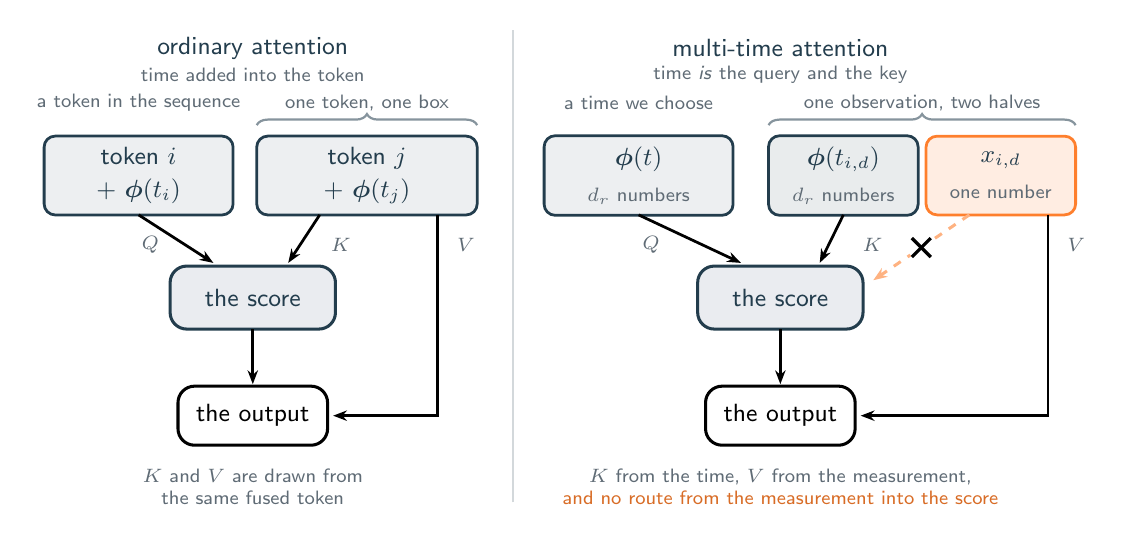
\begin{tikzpicture}[
    every node/.style={font=\sffamily},
    lab/.style={font=\sffamily\scriptsize, text=labelcolor},
    tag/.style={font=\sffamily\scriptsize, text=c2},
    hot/.style={font=\sffamily\scriptsize, text=c3!85!black},
    ttl/.style={font=\sffamily\small, text=c2},
    fused/.style={rectangle, rounded corners=4pt, draw=c2, fill=c2!8, text=c2,
                  line width=1.0pt, minimum height=1.0cm, font=\sffamily\small,
                  align=center, inner sep=4pt},
    keybox/.style={rectangle, rounded corners=4pt, draw=c2, fill=c2!10, text=c2,
                   line width=1.0pt, minimum height=1.0cm, font=\sffamily\small,
                   align=center, inner sep=4pt},
    valbox/.style={rectangle, rounded corners=4pt, draw=c3, fill=c3!14, text=c2,
                   line width=1.0pt, minimum height=1.0cm, font=\sffamily\small,
                   align=center, inner sep=4pt},
    sc/.style={rectangle, rounded corners=6pt, draw=c2, fill=c4, text=c2,
               line width=1.1pt, minimum width=2.1cm, minimum height=0.80cm,
               font=\sffamily\small},
    outbox/.style={rectangle, rounded corners=6pt, draw=c1, fill=white, text=c1,
                   line width=1.1pt, minimum width=1.9cm, minimum height=0.75cm,
                   font=\sffamily\small},
    arr/.style={-{Stealth[length=5pt]}, line width=1.0pt, color=c1},
    ghost/.style={-{Stealth[length=5pt]}, line width=1.1pt, color=c3!60, dashed},
]

\draw[c2!20, line width=0.8pt] (6.40, 0.35) -- (6.40, 6.35);

\node[ttl] at (3.10, 6.12) {ordinary attention};
\node[lab] at (3.10, 5.78) {time added into the token};
\node[ttl] at (9.80, 6.12) {multi-time attention};
\node[lab] at (9.80, 5.78) {time \emph{is} the query and the key};

% ================================================================ left panel
\node[lab] at (1.65, 5.42) {a token in the sequence};
\node[fused, minimum width=2.4cm] (lq) at (1.65, 4.50)
     {token $i$\\[1pt] $+\ \boldsymbol{\phi}(t_i)$};

\node[fused, minimum width=2.8cm] (lk) at (4.55, 4.50)
     {token $j$\\[1pt] $+\ \boldsymbol{\phi}(t_j)$};
\draw[decorate, decoration={brace, amplitude=4pt}, c2!55, line width=0.8pt]
     (3.15, 5.14) -- (5.95, 5.14);
\node[lab] at (4.55, 5.42) {one token, one box};

\node[sc]     (ls) at (3.10, 2.95) {the score};
\node[outbox] (lo) at (3.10, 1.45) {the output};

\draw[arr] (1.65, 4.00) -- (2.60, 3.39);
\node[lab] at (1.80, 3.62) {$Q$};
\draw[arr] (3.95, 4.00) -- (3.55, 3.39);
\node[lab] at (4.22, 3.62) {$K$};

\draw[arr] (5.45, 4.00) -- (5.45, 1.45) -- (4.12, 1.45);
\node[lab, anchor=west] at (5.57, 3.62) {$V$};

\draw[arr] (3.10, 2.55) -- (3.10, 1.85);

\node[lab, anchor=north, align=center] at (3.10, 0.90)
     {$K$ and $V$ are drawn from\\ the same fused token};

% =============================================================== right panel
\node[lab] at (8.00, 5.42) {a time we choose};
\node[fused, minimum width=2.4cm] (rq) at (8.00, 4.50)
     {$\boldsymbol{\phi}(t)$\\[2pt] {\scriptsize\color{labelcolor}$d_r$ numbers}};

\node[keybox, minimum width=1.9cm] (rk) at (10.60, 4.50)
     {$\boldsymbol{\phi}(t_{i,d})$\\[2pt] {\scriptsize\color{labelcolor}$d_r$ numbers}};
\node[valbox, minimum width=1.9cm] (rv) at (12.60, 4.50)
     {$x_{i,d}$\\[2pt] {\scriptsize\color{labelcolor}one number}};
\draw[decorate, decoration={brace, amplitude=4pt}, c2!55, line width=0.8pt]
     (9.65, 5.14) -- (13.55, 5.14);
\node[lab] at (11.60, 5.42) {one observation, two halves};

\node[sc]     (rs) at (9.80, 2.95) {the score};
\node[outbox] (ro) at (9.80, 1.45) {the output};

\draw[arr] (8.00, 4.00) -- (9.30, 3.39);
\node[lab] at (8.16, 3.62) {$Q$};
\draw[arr] (10.60, 4.00) -- (10.30, 3.39);
\node[lab, anchor=west] at (10.72, 3.62) {$K$};

% the route the measurement does not have
\draw[ghost] (12.20, 4.00) -- (10.98, 3.17);
\fill[white] (11.59, 3.585) circle (0.17);
\draw[c1, line width=1.2pt] (11.47, 3.705) -- (11.71, 3.465);
\draw[c1, line width=1.2pt] (11.47, 3.465) -- (11.71, 3.705);

\draw[arr] (13.20, 4.00) -- (13.20, 1.45) -- (10.82, 1.45);
\node[lab, anchor=west] at (13.32, 3.62) {$V$};

\draw[arr] (9.80, 2.55) -- (9.80, 1.85);

\node[lab, anchor=north, align=center] at (9.80, 0.90)
     {$K$ from the time, $V$ from the measurement,\\
      \textcolor{c3!85!black}{and no route from the measurement into the score}};

\end{tikzpicture}
\end{document}
